\documentclass[sotsuron]{kuee}
\usepackage[dvipdfmx]{graphicx}

\title{チームスポーツの戦術改善に資する選手向け可視化システムの開発}
\author{今井 晨介}
\professor{小山田 耕二 教授}
\course{京都大学工学部}
\department{電気電子工学科 電気工学専攻}
\date{平成27年2月13日}

%%% 本文
\begin{document}
\maketitle	
\tableofcontents


%%%序論
\chapter{序論}
	近年、ビッグデータを用いた視覚的分析の需要が高まっており、スポーツの分野でも様々な手法が提案されている。スポーツ分野における既存の視覚的分析補助システムは、試合のデータを用いたデータマイニングを支援し、主に監督、コーチ、または記者をユーザー対象としている。
	特に、プロの監督、コーチは試合での戦術戦略に関する意思決定を行う際に視覚的分析補助システムを用いていることがあり、その需要に合ったシステム研究も行われている[cite]。
	また、記者がスポーツに関する記事を書く時、出来得る限り偏った表現をしないように補助するスポーツ可視化分析システムの開発も行われている[cite]。
	しかしながら、選手自らが戦術、戦略を練るチームや、選手自らの分析が試合に大きく影響するスポーツの場合、上記の既存のスポーツ分析システムの多くは選手が頻繁に利用することを想定していないものが多く、操作が複雑、もしくは表現が難解であり、分析に時間を要する事が多い。
	\\例えば、選手自らが戦術、戦略を練ることが多く、選手個人の戦術理解が重要な男子ラクロスというスポーツの場合、監督やコーチのみならず、選手自らもビデオを観ることで出場した試合を分析し、その試合に用いられた戦術戦略はいかに機能したか、選手たちのコンディションはどうだったのかを振り返り、以後の戦術改善に活かすことが多い。また、これから対戦をする相手チームに勝つための戦術を練る際に、相手のプレーをビデオで観る、もしくは試合データを視ることで分析を行うこともある。これらすべての分析を処理するの多くの時間を費やしているのが現状である。
	練習やトレーニングに時間を割かなければいけないスポーツ選手にとって、分析に要する時間は非常に負担である。
	にもかかわらず、選手たちが日々利用することを想定し、彼らの試合分析方法に最適化した、多くの時間を費やさず、戦術改善し資す分析を可能にするシステム開発に関する先行研究は見受けられない。
	\\そこで、本研究では既存システムの複雑さを解消し、視覚的に分析を行えるようにすることで、試合分析にかける時間を軽減し、選手たちが容易に利用でき、かつ有益な情報を得ることが可能なスポーツ可視化システムを開発した。
	まずはじめに、システム開発に際して本研究では、選手の利用を想定した分析補助ツールの需要を調査し、その必要性を確認した。
	加えて、本提案システムへの要望調査では、評価グリッド法[]とアンケート手法を用いて、要求要項を明確にし、システム実装を行った。
	本提案システムはダッシュボードフレームワークを改良し、選手利用に最適化している。
	以降、本提案システム概要の紹介に際して、分析ツールのメイン画面をダッシュボードと呼称する。
	本提案システムでは、ダッシュボード上に複数のパネルを配置でき、各パネルにそれぞれゲームに関する情報を視覚化したグラフとともに表示する。
	また、ダッシュボードに下記の機能を加えることで、選手たちは容易に利用でき、戦術改善に有益な情報を得ることができた。
		\begin{itemize}
			\item 結果の善し悪しによってパネルの配置、配色を変えることで情報探索補助する機能
			\item パネル間の比較補助機能
			\item インタラクティブに情報探索を行える機能
			\item 特定のプレーを動画にて確認する機能
			\item 試合を俯瞰する機能
		\end{itemize}
	ただし、本論文での有益な情報とは、例えば、「どのプレーで負けていたのか、もしくは勝っていたか。」「どのようなプレーをしていたから勝っていたのか、負けていたのか。」「相手チームの誰が要注意人物であるか。」などの選手にアンケート調査を行って要求の高かった項目のことである。
	また、上でいうシステムの容易性とは、選手に対して調査を行った際に要望として高かった「システムの扱いやすさ」、「グラフのイメージしやすさ」、「分析時間を短縮できるシステムの優れた情報探索能力」である。
	\\本論文の構成は以下のとおりである。
	第1章は、本論文の序論である。第2章は、本論文の関連研究を挙げ、第3章では本提案システムの要求要項の抽出について述べる。
	第4章ではシステム実装について説明し、第5章では本提案システムの評価実験について述べる。
	第6章では本論文の結論と今後の展望について述べる。

%%%関連研究
\chapter{関連研究}
	本章では、スポーツに関する可視化分析システム、及び本提案システムで採用したダッシュボード形式の可視化分析システムについて、本論文での関連研究を述べる。
	\\Charlesらは、サッカーストーリーというシステムを開発した。
	このサッカーの分析ツールを用いることで、サッカーの練習効率を上げ、正しい分析によるコミュニケーションを促すことができるとCharlesらは述べている。
	サッカーストーリーでは1つずつゲームを俯瞰し、また詳細をも見ることができる。
	サッカーストーリーを用いることで、記者は試合について記事を書く時に、監督は試合について分析する時に従来より時間を短縮できるようになると主張している。
	サッカーストーリーでは一つの試合での出来事をフィールド上にグラフを配置することで、その試合のダイジェストを視覚的に得ることができる。
	しかしながら、試合間のデータの比較を行えない点で不便さがある。
	\\Tomらは、これまでに研究されているテニスの可視化技術は、プロ選手の試合放送の質を高め、コーチが選手をコーチングするために、ボールや選手のトラッキングデータを用いることに終始している事に注目した。
	Tomらはデータの収集はコストがかかることを考慮し、データを手入力できるためアマチュアでも低コストで分析可能なシステムを考案した。
	本提案システムでも、手入力可能なデータを可視化している。
	スコアや、ラリーの長さや、サーブの情報や、試合のビデオなどをコンシューマ向けビデオカメラから簡単に試合データを収集し、Tomらの開発したtennivisシステムにより3種の手法を用いている。
	Tennis visシステムを用いることでテニスのコーチ、プレーヤーは試合のパフォーマンスを素早く振り返ることができると主張している。
	しかしながら、サッカーストーリーと同様、試合間のデータの比較には不便さが存在する。
	\\Kristらは、イベントの流れを視ることができるoutflowシステムを開発した。
	Outflowシステムでは特定のイベントフローデータに対しての可視化手法としては優れており、容易にフローの結果を知ることができ、複数の試合の俯瞰する機能としては優れている。
	複数の試合を俯瞰する機能は本提案システムでは、Outflowのようにフローで視るのではなく、ボタン選択によって行っている。	
	\\上記のすべてのスポーツ可視化システムは、選手も利用対象であるとは述べつつも、実装段階、評価段階において選手の意見は含まれていない。
	選手自らが戦術、戦略を練るチームや、選手自らの分析が試合に大きく影響するスポーツの場合、こういった既存のスポーツ分析システムの多くは選手の利用を想定しているとはいいつつも、操作が複雑、もしくは表現が難解であり、分析に時間を要する事が多い。
	また、評価実験に際して、定量的な評価を行わず数名の専門家に対して定性的な意見を得ることに終始しているものが多く、必ずしも有用性が明らかとは言えない。
	\\したがって、本論文では利用想定者を幅広くせず、あえてターゲットを選手のみに絞り、選手の目線で必要な要素を考慮して可視化システムを作成している。
	\\Arunらは、レイアウト変更可能なダッシュボードフレームワークを作成した。
	Arunらの提案しているダッシュボードフレームワークは、レイアウト変更可能なダッシュボード上でのデータ可視化プロセスの自動化をできるよう開発した。
	このフレームワークではデータの種類には依存せず、また、ユーザー好みの構成にもとづいてグラフを生成することができ、サードパーティ製やチャートライブラリを用いたグラフの生成が可能であり、柔軟も合わせ持っている。
	\\本提案システムでは、既存のダッシュボードフレームワーシステムを参考にしつつ、選手たちの要望に沿ったダッシュボードシステムを作成した。

%%%本提案システム
\chapter{本提案システム}
	\section{システム設計}
		選手が容易に利用可能なシステムの条件を明らかにするため、選手に対してアンケート調査を実施した。
		アンケート調査を実施する前段階に、アンケート質問項目を検討するにあたり、評価グリッド法による予備調査を行った。
		\subsection{評価グリッド法による予備調査}
			ラクロス可視化ツールへの要望を洗い出すために、評価グリッド法によるインタビュー調査を行った。
			\subsubsection{評価グリッド法}
				評価グリッド法ついての概要を説明する。
				説明できねーwwwww
				%評価グリッド法は、讃井らが提案した定性評価手法であり、一人ひとりに対してインタビューを行う。
				%まず評価対象となりうるエレメントを複数提示し、それらエレメントを比較し良い部分を抽出する。
				%次に、抽出したオリジナル評価項目の上位項目と下位項目を答えてもらい、グラフにマッピングする。
				%ここで言う上位項目とはオリジナル評価項目を挙げた理由であり、オリジナル評価項目について「〇〇だとなぜいいのですか」と質問を行う。この作業をラダーアップと呼称する。
				%またこれとは逆に、下位項目はオリジナル評価項目を挙げるにあたり、「具体的にどういうところが〇〇なのか」と質問を行う。この作業をラダーダウンと呼称する。
				%ラダーアップとラダーダウンを合わせてラダリングと言い、ラダリングされた項目について再度ラダリングを行ない、対象者の回答が引き出せなくなった時点でインタビューを終了する。
				%これらオリジナル評価項目とラダリングされた項目をマッピングすることで視覚的に認識しやすいグラフが作成される。
				%以上の手法を取ることにより、評価グリッド法は認知心理学的の立場から人々のある対象に対する評価を明らかにし、深層心理を引き出すことができるとされている。
				%従って、評価グリッド法は調査対象全体の価値観を把握するのに有効な手段であり、本調査では選手向け可視化ツールの要望を把握する手段として最適と考え、採用した。[][][]
			\subsubsection{調査方法}
				京都大学男子ラクロス部に協力して頂き、5名に対して評価グリッド法に沿ったインタビューを行った。
				まず、尾上らの開発するE-gridを用いて1人ずつインタビューを行い、評価構造を図を作成した。
				オリジナル評価項目として、同部で利用されていた表計算アプリケーションフォーマットの表データと、ラクロス可視化システムのプロトタイプを用いてラダリングを行った。
				ラクロス可視化システムプロトタイプとして、ラクロスにおけるある二つのプレーに関して、フィールド図上にプロットしたグラフを提示した。
				この5人の評価構造図を、項目の重複をマージすることにより一つの評価構造図にまとめた。
			\subsubsection{調査結果}	
				調査で得られたグラフを図~\ref{fig:egrid}に示す。
					\begin{figure}
						\begin{center}
							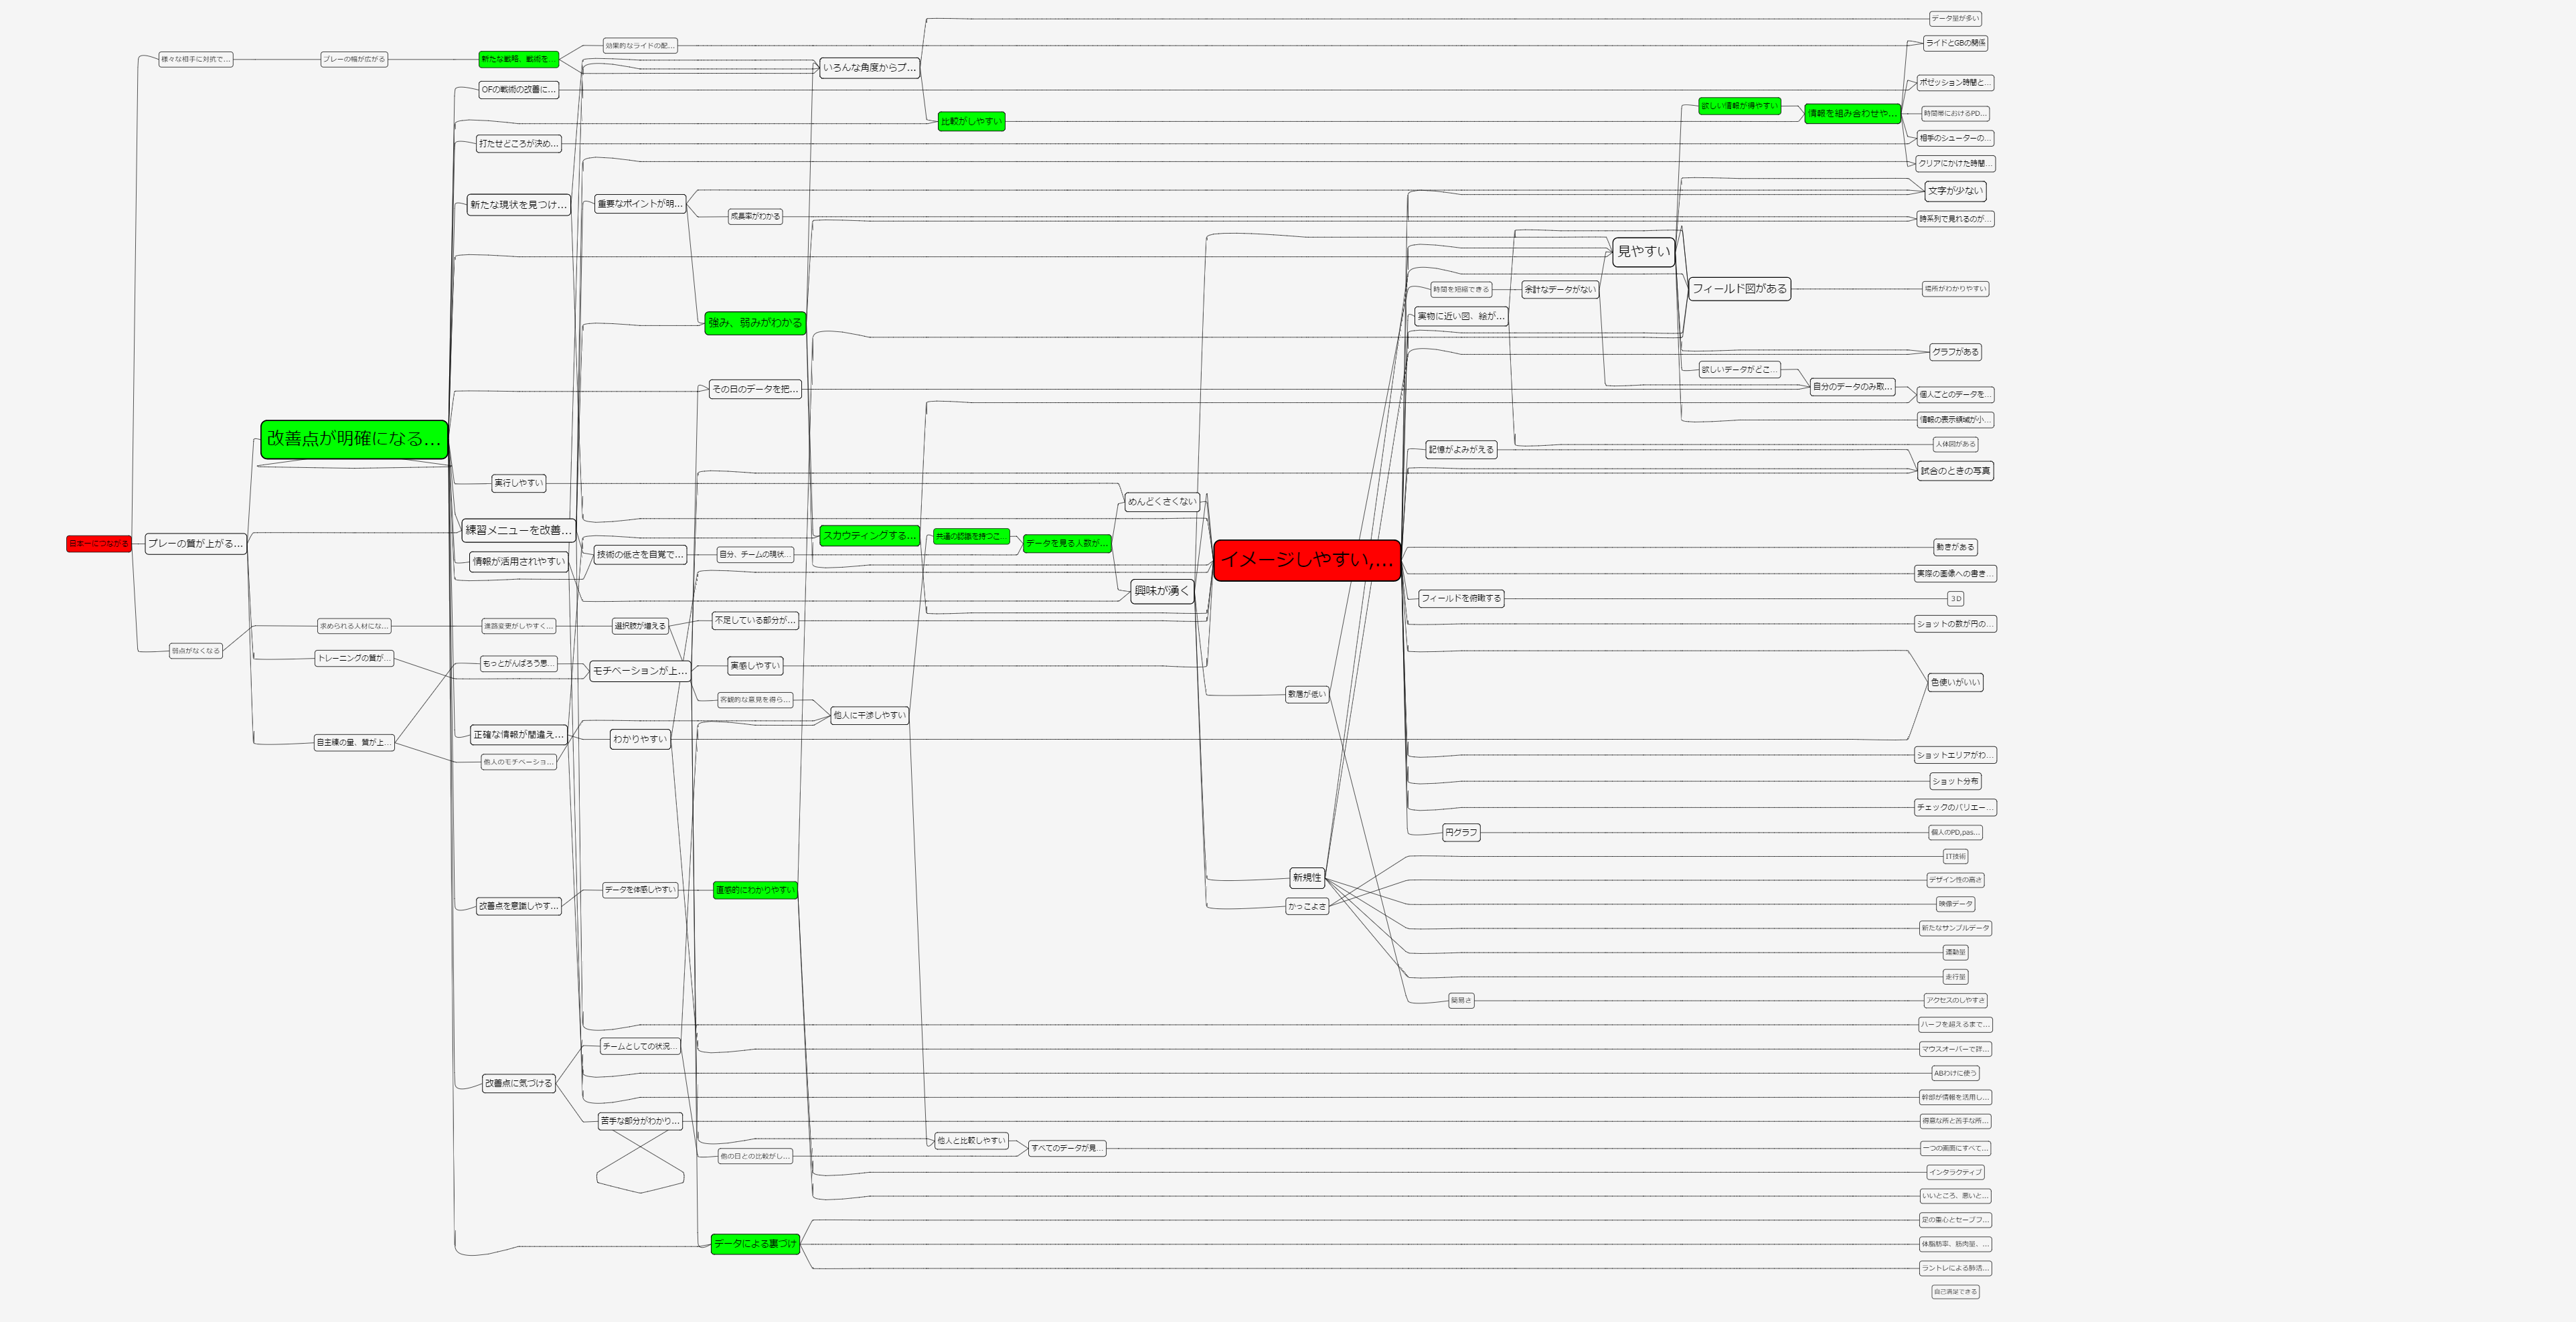
\includegraphics[angle=90,width=20cm]{egrid.eps}
						\end{center}
						\caption{評価構造図}
				  		\label{fig:egrid}
					\end{figure}
			\subsubsection{調査考察}
				本調査で得られたネットワーク図からアンケート質問項目を抽出し、インタビューに際して選手たちに共通していた分析に関する意見についてまとめる。
				\paragraph{アンケート項目の抽出}
					評価グリッドインタビューを行った結果、下位項目に、選手たちが知りたい具体的なプレー結果が何であるかを読み取れた。
					また、上位項目には、「こんな感じであってほしい」といったシステム概要への抽象的な要望が多かった。
					アンケート質問項目については、次項にて詳細を記述する。
				\paragraph{選手たちの共通意見}
					選手が共通して強く望んでいた一つが、分析システムの容易性であった。
					容易性とは具体的に「システムの扱いやすさ」、「グラフのイメージしやすさ」、「分析時間を短縮できるシステムの優れた情報探索能力」などのことである。
					彼らスポーツ選手は、練習、トレーニングに加え、ビデオによる戦術分析に多くの時間を割いており、負担を感じていた。
					戦術分析は必要な要素ではあるので欠かせないが、表計算アプリケーションを用いた試合情報の集計では戦術分析に活かせておらず、試合のすべてのビデオを見直すことで戦術分析を行っていると述べていた。
					そこで、これまでより容易に利用可能な、可視化技術を用いた分析補助システムの実用化を望んでいた。
					したがって本調査により、序論で述べていた、スポーツ現場における本提案システムのニーズを確認した。
		\subsection{アンケート調査}
			\subsubsection{調査方法}
				評価グリッド法によるインタビューではシステムへの要求項目として数が多く、優先度が明確ではないので、評価グリッド法の結果からアンケート質問項目を作成し、同部に対してアンケート調査を行ない、システム要件項目を明確にした。
				\\システム概要の要望に関する質問項目は評価グリッド法より15項目を抽出した。
				選手が分析したい対象に関する質問項目も、評価グリッド法より35項目を抽出した。
				また、両項目とも複数選択を可とした。
				システムの利用用途、目的に関する質問は自由回答とした。
				\\アンケート項目詳細は付録に記載する。
			\subsubsection{調査結果}
				同部より78名の回答を得た。アンケート結果を以下に示す。
				\begin{itemize}
				\item システム概要に関する回答で、選択数の割合が全体回答者数の25\%以上であった項目を挙げる。
					\begin{enumerate}
					\item データを簡単に見ることができる。(43人、69\%)
					\item データの比較をすることができる。(37人、60\%)
					\item イメージしやすい。(32人、52\%)
					\item フィールド図で視覚化されている。(28人、45\%)
					\item グラフを用いている。(23人、37\%)
					\item 一つの画面にデータがまとめられている。(22人、35\%)
					\item 映像を含んでいる。(17人、27\%)
					\end{enumerate}
				\item 選手が分析したい対象に関する回答で、選択数の割合が全体回答者数の50\%以上であった項目を挙げる。
					\begin{enumerate}
					\item ショット(46人、74\%)
					\item 1on1(39人、63\%)
					\item グラウンドボール(34人、55\%)
					\item 選手の動き(33人、53\%)
					\item クリア(32人、53\%)
					\item パス(31人、50\%)
					\item 得点(31人、50\%)
					\end{enumerate}
				\item システムの利用用途、利用目的に関する質問の回答は、重複が多かったものを挙げる。
					\begin{enumerate}
					\item 対戦相手チームの特徴を把握し、自チームの戦術を練るため。
					\item 試合後に、自チームの反省を行ない、以後の方針を決定するため。
					\item 結果の良かったエレメントと、悪かったエレメントの違いを見出し、新たな視点を得るため。
					\item 試合に出るレギュラーを選定する材料とするため。
					\item データの蓄積を行うことで、最適な戦術を選び出すため。
					\end{enumerate}
				\end{itemize}
			\subsubsection{調査考察、システム要件要項}
				評価グリッド法を用いたインタビュー調査とアンケート調査により、具体的なシステム要件を洗い出された。
				評価グリッド法を用いることで、精査されたアンケート質問項目が作成され、質問項目に漏れの少ないアンケート調査を行う事により、アンケートのみの調査に比べると、正確な選手の要望を確認出来たと考えられる。
				\begin{itemize}
					\item システム概要に関する回答についての考察
						\begin{description}
							\item [「データを簡単に見ることができる。」:]
							評価グリッド法インタビューで多く聞かれた、分析にかける時間短縮を望んでのことだと考えられる。
							従って要項としては、時間短縮のためにデータへのアクセスビリティを考え、webアプリケーションによる実装を行った。
							同様に下項目と重複するが、視覚的に認識することが可能にすることで、時間短縮を図った。
							また、簡単さという表現から、アプリケーションのわかりやすい操作性も求められていると考えられるので、選手にわかりやすユーザーインターフェイスを実装した。
							\item [「データの比較をすることができる。」:]
							他人、他チーム、他日時とのデータの比較を容易にするべく、本論文で提案するパネルベースのシステム構築を行った。一つのデータのまとまりを一つの「パネル」の中で表現し、複数の「パネル」を画面上に配置し、パネル間の比較を補助する機能を実装した。
							\item [「イメージしやすい。」:]
							可視化技術を用いることにより、ユーザーが生データより認識しやすいグラフを提示する。
							\item [「フィールド図で視覚化されている。」:]
							上の「イメージしやすい」という項目の具体的手段にあたると考えられる。本提案システムでは、「イメージしやすい」グラフを作成するため、積極的にフィールド図を用いて実装を行った。
							\item [「グラフを用いている。」:]
							当項目に関しても、上二項目の具体的手段であると考えられ、本提案システムでは、積極的にグラフを用いてデータの視覚化し、システム実装を行った。
							\item [「一つの画面にデータがまとめられている。」:]
							データ表示ページが複数の画面に分断されているシステムの場合、ページ遷移により理解の妨げになると考えられる。従って、本提案システムでは一つの土台を上に「パネル」を配置する方式を提案する。本論文では、この土台を「ダッシュボード」と呼称する。
							\item [「映像を含んでいる。」:]
							ユーザーが詳細に観たいプレーについては、グラフ上のプロット等を選択することによりインタラクティブに動画を再生できるよう実装した。
						\end{description}
					\item 選手が分析したい対象に関する回答についての考察
						\\回答で得られた7項目より以下の4つのグラフを作成した。詳細については次項で述べる。
							\begin{itemize}
								\item Ground ball
								\item Shots
								\item Score
								\item Ballmove
							\end{itemize}
					\item システム利用用途、利用目的に関する回答についての考察
						\\システム利用用途として様々なエレメントの比較と、試合の俯瞰の要素が求められていると考えられる。
						従って、エレメントの比較と、試合の俯瞰を補助する機能を実装した。
						以上より、システムの特徴的な機能を以下にまとめる。
						\begin{enumerate}	
							\item 試合を俯瞰する機能
							\item 結果の善し悪しによってパネルの配置、配色を変えることで比較分析を補助する機能
							\item インタラクティブに情報探索を行える機能
							\item 特定のプレーを動画にて確認する機能
						\end{enumerate}
				\end{itemize}
	\section{システム実装}
		\subsection{ダッシュボード}
			本提案システムメイン画面はダッシュボードと呼称し、ユーザーの操作によりこのダッシュボード上にパネルを配置していく。(Fig)
			パネルにはひとつのグラフを表示し、プレーに関するデータを視覚化した。
			ダッシュボード上部にナビゲーションバーを配置しており、本提案システムに搭載している機能は、このナビゲーションバーから選択することで利用できるようにした。
			ダッシュボードにてユーザーが主に行う操作は対象試合を選びパネルの配置することと、配置されたパネル間の比較することであり、複雑なズーミングやわかりにくいフィルタリングは行わずに扱えるようにした。
		\subsection{システム起動}
			本提案システムは、web技術を用いて実装した。
			アプリケーションを起動する際、スマートフォン、タブレット、電子計算機などの電子端末であれば、ほぼすべてに搭載されているwebブラウザにてアプリケーションを実行することが可能である。
			専用アプリケーションのインストールや、データファイルのダウンロードの必要がなく、この実行環境ユーザーの要望する容易性に応える要素となる。
		\subsection{パネルの選択}
			本提案システムでは、セレクションモーダル画面にて、これまでのすべての試合を探索できるようにした。
			本システムの起動時、もしくはナビゲーションバーから「graph」を選択することで	、セレクションモーダル画面に移行する。
			ユーザーは見たい試合を探し、チームのボタンを押すことで、ダッシュボード上にパネルが生成される。
			セレクションモーダルに3つのタブを備え、目的に応じてタブを使い分けられるようにした。
			ゲームタブでは、フィルタリング機能を備えているため、特定のキーワードから試合を探索でき、チームを選択することで、全データから絞り込むことができるようにした。(Fig)
			チームタブでは、試合の点数差によって選択ボタンの配色を変えており、特定のチームのこれまでの試合状況の俯瞰を可能にした。(Fig)
			グラフタブでは試合ではなく、パネルを直接選択する。複数のパネルを選択することができ、またフィルタリング機能を備えているため、試合間でのデータ比較が容易に行えるようにした。(Fig)
		\subsection{パネル}
			セレクションモーダル画面よりダッシュボード上に生成されたパネルについて詳細を述べる。
			パネルでは二つのタブを開けるようになっており、ひとつのタブにはパネルの主目的である、プレーに関するグラフを表示しており、もうひとつにはパネルの詳細情報を表示するようにした。詳細情報とは選択された試合の詳細な記述である。
			要素の種類としては4種類の実装を行った。グラフ生成にはJavaScript,D3jsライブラリを用いた。
			Ground ball
			Figに示すように、フィールド図上にグラウンドボールをスクープした選手をプロットした。対象チームを青、対戦チームを赤とし、プロット点内にスクープした選手の背番号を表記した。また、エリアごとにチームのスクープ頻度を色分けし、視覚的に勝負を分析する補助を加えた。
			プロットした選手をブラウザにてタッチすると、その時間の動画再生できるようにした。
			Shots
			Figに示すように、ショットグラフは2つの要素から構成した。ひとつはフィールド図、もうひとつはゴール図である。
			フィールド図ではショットを打った方法と場所をプロットした。またショットの3種の結果、ゴール、アウト、セーブをプロットの色で分けた。対象試合での全体的なショット結果を視覚的に表記し、この分布プロットから対象チームのショットに関する傾向と成功率を解釈できるようにした。
			ゴール図では、対象チームのショットの分布をプロットした。フィールド図と同様にショットの結果を色分けプロットした。この分布プロットから対象チームのショットに関する傾向と成功率を解釈できるとともに、相手ゴーリーの得手不得手を分析することを可能にした。
			Score
			Figに示すように、対象チームでの得点者に関して分析できるようにし、インタラクティブな棒グラフと円グラフにより視覚化した。
			この棒グラフと円グラフは相互に関連しており、棒グラフには対象チームの選手の総ショット数を表示し、ある選手を選択すると、その選手のショットの内訳が円グラフに表示されるようにした。また、円グラフには対象チームの総ショット内訳を表示し、一つのショット要素を選択すると、そのショット要素の内訳選手が棒グラフに表示されるされるようにした。
			Ballmove
			Figに示すように、対象チームの試合中の動きと試合の展開を視覚的に視ることができるようにした。
			Ball moveはフィールド図と試合展開図の二つのグラフより視覚化した。
			試合展開図では、試合の状況について横軸は時間を取り、縦軸は試合状況を取った。
			この試合展開図により試合状況を俯瞰して視ることができ、詳細に視たい場合は、Figのように範囲を指定することで詳細を確認できる。
			また、フィールド図において、試合展開図にて範囲を指定すると、その時間内でのボールの動きと、ボールの動きに関わった選手が表示される。
			このグラフにより、「1on1」、「選手の動き」、「クリア」、「パス」を分析対象とすることができる。

		\subsection{ダッシュボードファンクション}
			本提案システムのダッシュボードに搭載されている機能について述べる。ダッシュボードファンクションはナビゲーションバーから選択できる。
			\subsubsection{レイティング機能}
			パネルにはプレーに関するグラフが表示されるが、そのプレーの良し悪しをパネルの色によってわかるようにした。
			パネルの色はユーザーが任意に色を設定できるようにした。
			この配色機能により、ある試合のデータについてダッシュボードにパネルを出力すると、試合中の良い箇所、悪い要素を一目で理解できるようにした。
			あるチームのあるプレーの変化を知りたい場合にも、この機能を利用することで経過を視ることができるようにした。
			\subsubsection{ソート機能}
			パネルの配置順序はパネルタイトルバーもしくはダッシュボードファンクションの一つであるソート機能により変更できるようにした。
			ソート機能はパネルのデータに従って自動的に配置順序をソートできるようにした。
			日時、プレーの良し悪し等によりソートを行えるようにした。
			\subsubsection{メモ機能}
			パネルは基本的にグラフを表示する役割であるが、ユーザーによりパネル内にメモを加える事ができるようにした。
			ユーザーがメモを加えられることにより、分析の補助を狙った。
			\subsubsection{最小化機能}
			パネルのタイトル、もしくはコラプスボタンを押すことでパネルを最小化できるようにした。
			パネル数が多くなる場合、スクロールして見るには見づらくなるため、この最小化可能な機能を加えた。


	\section{提案システムを用いた利用手順}
		\begin{enumerate}
			\item システムの立ち上げ
				\\Figに示すように、ブラウザに指定URLを打ち込み、webアプリケーションを立ち上げる。
				アプリケーションを起動する際、スマートフォン、タブレット、電子計算機などの電子端末であれば、ほぼすべてに搭載されているwebブラウザにてアプリケーションを実行することが可能である。専用アプリケーションのインストールや、データファイルのダウンロードの必要がなく、この実行環境の容易性はユーザーの要望に応える要素となる。
			\item データの選択
				\\Figの画面にて、知りたい情報を選択する。
				この際、蓄積されているすべてのデータを取り出すことが可能であり、それらすべてのデータを探索できるダッシュボード機能を実装した。
				Figでは、これまでの試合すべてを俯瞰でき、キーワードを入力することで、取り出したい試合をフィルタリングすることができる。
				選択ボタンを押すことで、その試合でのすべてのデータがダッシュボード上にパネルが出力される。
				Figでは、対象チームを選択することで、その対象チームの試合のみ抽出でき、試合の戦績により配色を変えることで結果の良し悪しを容易に見分けるための情報探索補助を実装した。
				選択ボタンを押すことで、そのチームのすべてのデータがダッシュボード所にパネルが出力される。
				Figでは、すべてのパネル要素を選択できる。あるプレーに注目して観たい場合に、フィルターを利用して対象チームや、対戦相手、日時などで絞り、ボタンを選択しダッシュボードへパネル出力を行う。
				これらの機能を実装することで、様々な試合を俯瞰し、インタラクティブに情報探索を行えるようにした。
				\begin{figure}
					\begin{center}
						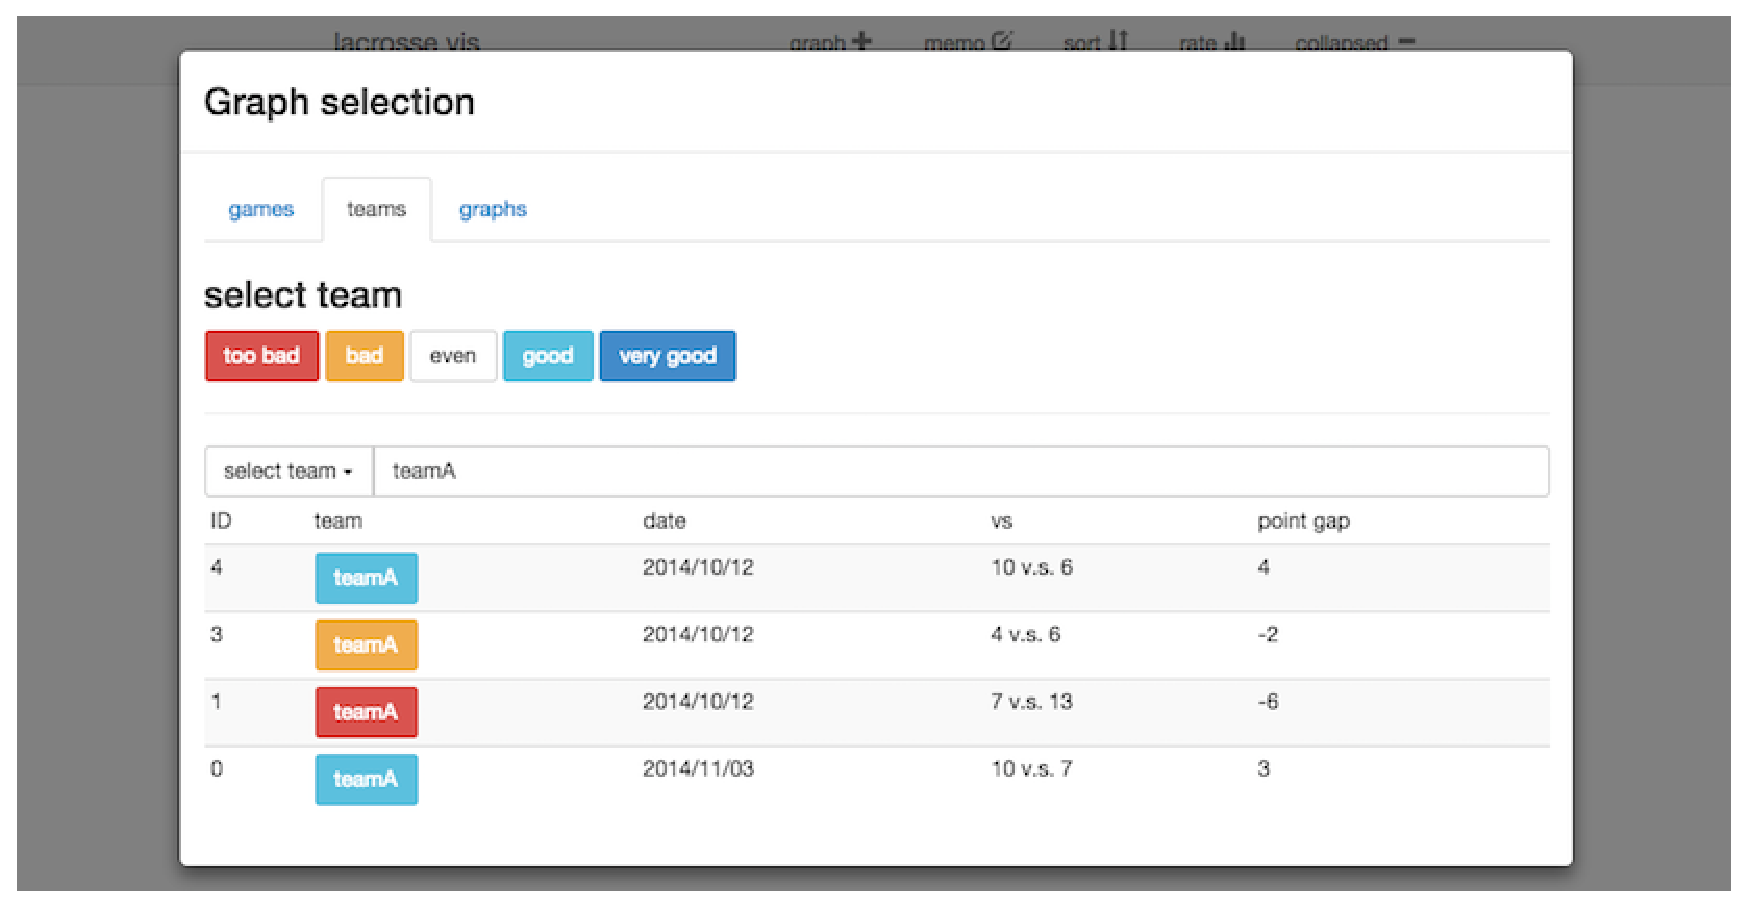
\includegraphics[width=\linewidth]{selection.eps}
					\end{center}
					\caption{選択画面}
			  		\label{fig:select}
				\end{figure}
			\item データの表示
				\\図で示すのように、手順2でパネルを出力することでダッシュボードにて、各要素のパネルが表示されるが、これらのパネル内では各要素のデータを視覚化グラフが表示されている。
				要素の種類としては4種類実装を行った。グラフ生成ツールにはD3jsライブラリを用いた。
				\begin{description}
					\item [Ground ball]
					Figに示すように、フィールド図上にグラウンドボールをスクープした選手をプロットした。対象チームを青、対戦チームを赤とし、プロット点内にスクープした選手の背番号を表記する。また、エリアごとにチームのスクープ頻度を色分けし、視覚的に勝負を分析する補助を加えた。
					プロットした選手をブラウザにてタッチすると、その瞬間の動画再生できるようになっている。
					\item [Shots]
					Figに示すように、ショットグラフは2つの要素から構成される。ひとつはフィールド図、もうひとつはゴール図である。
					フィールド図ではショットを打った方法と場所をプロットした。またショットの3種の結果、ゴール、アウト、セーブをプロットの色で分けた。対象試合での全体的なショット結果を視覚的に表記し、この分布プロットから対象チームのショットに関する傾向と成功率を解釈することができる。
					ゴール図では、対象チームのショットの分布をプロットした。フィールド図と同様にショットの結果を色分けプロットした。この分布プロットから対象チームのショットに関する傾向と成功率を解釈できるとともに、相手ゴーリーの得手不得手を分析することが可能である。
					\item [Score]
					Figに示すように、対象チームでの得点者に関して分析できる。Scoreは棒グラフと円グラフから構成されている。
					この棒グラフと円グラフは相互に関連しており、棒グラフには対象チームの選手の総ショット数を表示し、ある選手を選択すると、その選手のショットの内訳が円グラフに表示される。また、円グラフには対象チームの総ショット内訳を表示し、一つのショット要素を選択すると、そのショット要素の内訳選手が棒グラフに表示される。
					\item [Ballmove]
					Figに示すように、対象チームの試合中の動きと試合の展開を視覚的に視ることができる。Ball moveはフィールド図と試合展開図から構成される。
					試合展開図では、試合の状況について横軸は時間を取り、縦軸は試合状況を取った。
					この試合展開図により試合状況を俯瞰して視ることができ、詳細に視たい場合は、Figのように範囲を指定することで詳細を確認できる。
					また、フィールド図において、試合展開図にて範囲を指定すると、その時間内でのボールの動きと、ボールの動きに関わった選手が表示される。この機能により、「1on1」、「選手の動き」、「クリア」、「パス」を分析対象とすることができる。
					Figのように、パネルには複数のタブを実装した。
					タブを選択することで試合情報の詳細を確認できるようにした。これにより、グラフだけではわからないチームの詳細や、試合日時、試合場所等について確認できる。
					また、Figのようにパネルはグラフ以外にも、ユーザーが自由にメモを加える事もできる。
				\end{description}
			\item データの比較
				Figで示すのように、パネルの色を変更することができる。
				パネルの色をプレーの良し悪しによって決めることができる。また、ユーザーが任意に色を設定できる。この配色機能により、ある試合のデータについてダッシュボードにパネルを出力すると、試合中の良い箇所、悪い要素を一目で理解できる。あるチームのあるプレーの変化を知りたい場合にも、この機能を利用することで経過を視ることができる。
				またFigに示すのように、パネルの配置を変更することができる。
				配置変更機能により日付順、成績の良し悪しに配置を変更することができる。この配置変更によりパネル間の比較を支援する。
		\end{enumerate}

\chapter{評価実験}
	提案システムの有効性を検証するため、選手に対し評価実験を行った。
	本評価実験では以下の観点から提案システムの有効性について議論する。
	\begin{itemize}
		\item 選手が容易に操作可能なシステムであるか(NE比法)
		\item 従来のシステムに比べ、利便性は向上したのか(t検定)
		\item 選手が望む利用用途に即した情報探索が可能なシステムになっているか(アンケート調査)
	\end{itemize}
	以上の有効性を検証するために、同部15名に対してシステム評価実験を行った。
	\section{実験1}
		\subsection{評価方法}
			本提案システムが選手にとって容易に操作可能なシステムであるか、NE比法を用いて検証を行った。
			\\NE比法
			鱗原らによって開発されたNEM (Novice Expert ratio Method)[]は、行動データを定量的に分析することができる方法である。あるタスクを与え、開発者(エキスバート)と初心者ユーザ(ノービス)の操作に要する時間のギャップを比較し、システムの扱いやすさを示すことが可能である。
			あるタスクに対していくつかのステップに分割し、エキスパートとノービスのステップの時間差の比に注目することで、問題のあるステップを抽出することが可能である。
			\\NE比=T\_N/T\_E
			\\ T\_Nはエキスパートの操作時間であり、T\_Eはノービスの操作時間である。
			つまり、NE比が大きいステップは改善優先度の高いシステム要素であるといえる。
			有効性を示すために必要なノービスの数は15人であれば十分であると言われている。[]
			本実験では、利用目的の一つである「対戦相手チームの特徴を把握し、自チームの戦略を練る」場合を想定し、4つのステップを与え計測実験を行った。
			本評価においては2つの目的を持って操作を行うことを想定した。
			\\ひとつは、男子ラクロスではしばしば「最も得点を重ねる選手を封じる戦術」を取るので、この戦術を行うに際して必要な情報を探索するべく、「相手チームの最も得点を取る選手を探し出すこと」をタスクとして与えた。
			ただし今回のタスクでは、より正確に高得点者を洗い出すため、「試合におけるチーム間の得点差が大きい試合から探し出す」という条件を加えた。(この課題をタスク1とする。)
			\\もうひとつは、相手チームの弱点を見つけ出しその弱点をつくために、データから弱点を探すこととする。
			同上の試合から「相手チームの弱点を見つけ出す」タスクを与えた。(この課題をタスク2とする。)
			本評価実験では、評価実験のため試合のサンプルデータを10試合分作成し、用いた。
			ユーザーの操作をスクリーンキャプチャソフトを用いて録画し、実験終了後、本提案システムを用いたタスク処理に要した時間を計測した。
			数名づつ時間を分けて、提案システム使用方法を10分ほど説明したの後、計測実験を行った。
			図のように、1人ずつ計算機に向かってもらい、実験を行った。
			本評価での操作ステップを示す。
			\begin{enumerate}
				\item システムの立ち上げ(Fig)
				\\ブラウザを立ち上げる。
				ブックマークを選択して、Webアプリケーションを立ち上げる。
				\item データの俯瞰と選択(Fig)
				\\対戦チームをteamAとした時、teamAのこれまでの試合にて最も得点差の大きかった試合を選択し、ダッシュボード上にパネルを生成する。
				\item データ分析(Fig)
				\\パネル内をインタラクティブに操作し、高得点者を探し出す。
				タスク1が完了する。
				\item パネル間の比較(Fig)
				\\パネル間比較機能を用いて、相手チームの弱点を見つけ出す。
				タスク2が完了する。
			\end{enumerate}
			また、本提案システム開発者も同計測を行った。
		\subsection{評価結果}
			15名のノービスと、1名のエキスパートに対して実験を行った。
			ここで言うエキスパートとは、本提案システム開発者である。
			実験結果を図~\ref{fig:result01}に示す。
			図~\ref{fig:result02}ではステップに要したノービスの平均時間とエキスパートの時間、それぞれのステップのNE比を表している。
			\begin{figure}
				\begin{center}
					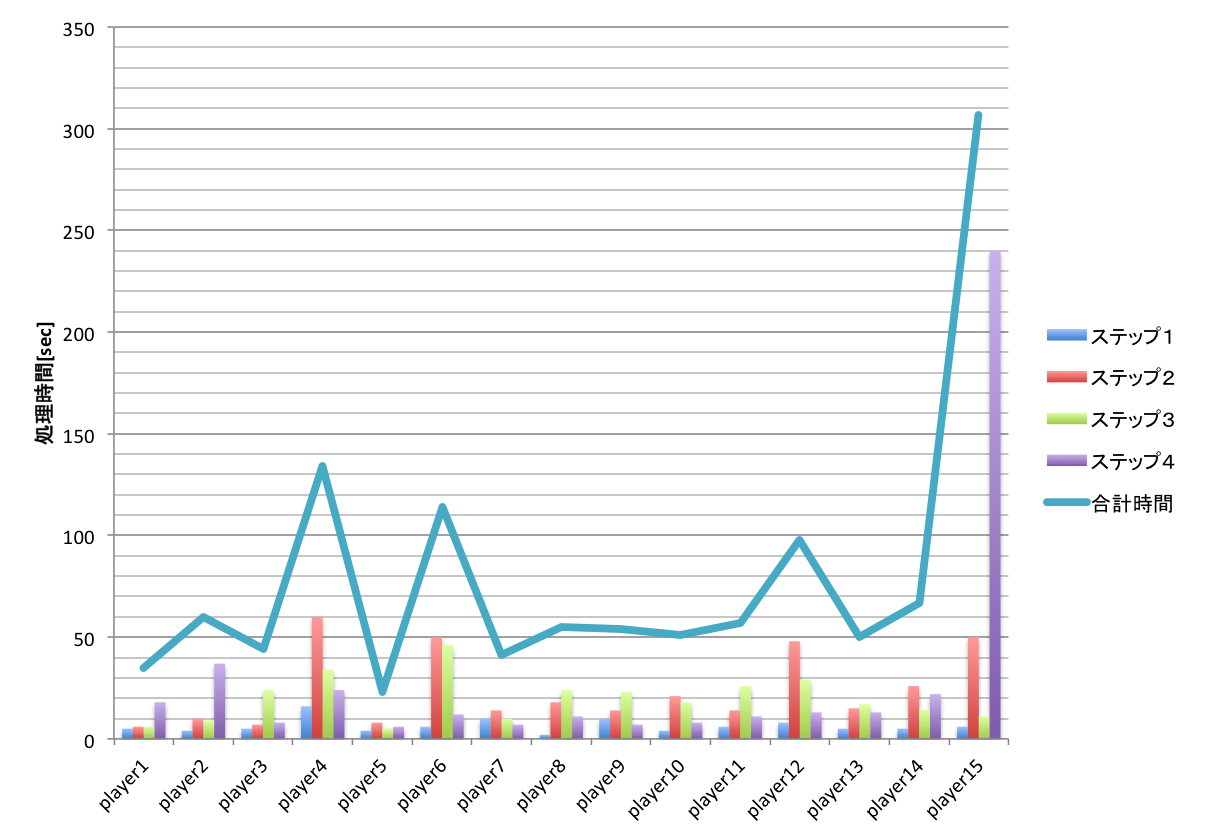
\includegraphics[width=\linewidth]{result01.eps}
				\end{center}
				\caption{本提案システムの操作時間}
		  		\label{fig:result01}
			\end{figure}
			\begin{figure}
				\begin{center}
					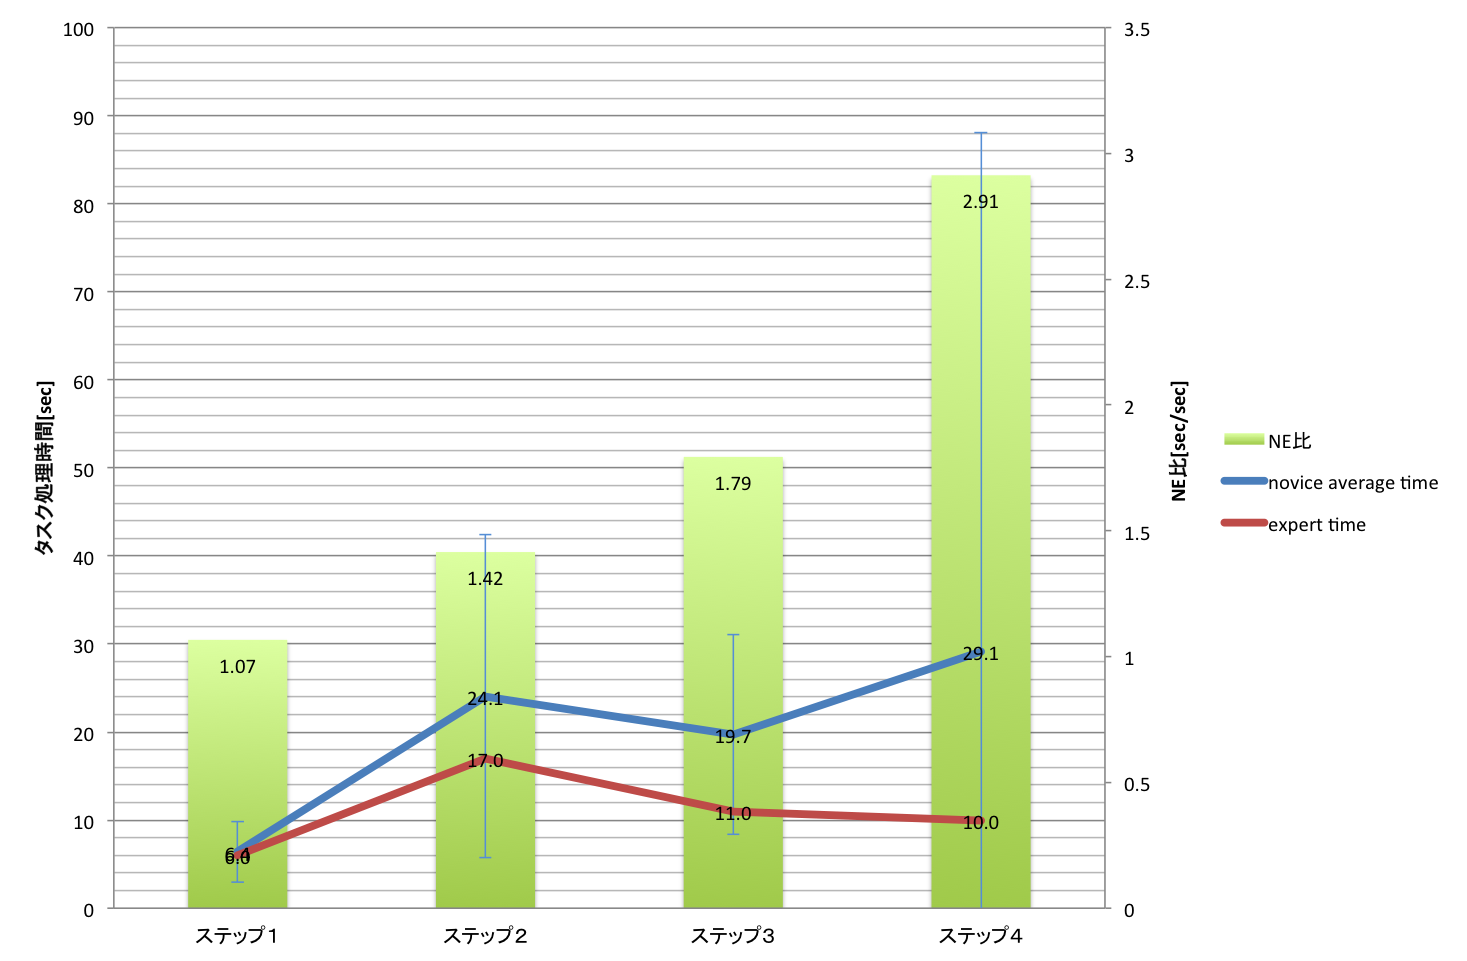
\includegraphics[width=\linewidth]{result02.eps}
				\end{center}
				\caption{NE比}
		  		\label{fig:result02}
			\end{figure}
		\subsection{評価考察}
			操作性について、一般的に、NE比4.5以上でなければシステムの操作性について問題がないといわれている。[]
			本実験では最大NE比は1.85であるので、本提案システムが選手にとって容易に操作可能なシステムであると言える。
			NE比が最も大きいステップ3に関しては「パネル内をインタラクティブに操作し、高得点者を探し出す」動作であるが、本著者が見ている限り、被験者は参照するべきグラフをわかったいるものの、どのようにインタラクションすればいいのか迷う場面が多く見られた。
			このステップ3の操作性に対する解決策としては、ユーザーの慣れと、インタラクション性の実装の見直しが考えられる。
	\section{実験2}
		\subsection{評価方法}
			同部での従来のシステムに比べ、利便性は向上したのかを検証するため、t検定を用いて評価した。
			NE比法と同様の方法にて、表計算アプリケーションを利用して「相手チームの最も得点差の大きかった試合での高得点者を探し出す」課題を与え、タスク処理にかかった時間をt検定を用いて本提案システムを用いた場合と比較することで、本提案システムの優位性を検証し、情報探索にかかる時間を削減出来るか試みた。
		\subsection{評価結果}
			実験結果を実験1の結果を加えて図~\ref{fig:result03}に示す。
			図~\ref{fig:result04}では各々のタスク処理時間と、利用アプリケーションの平均時間を記している。
			また、各ステップでの平均処理時間と、その標準偏差誤差範囲をエラーバーにて記している。
			図~\ref{fig:result05}では同部での各々の表計算アプリケーション利用状況と、表計算アプリケーションでの分析に要する処理時間について記している。
			\begin{figure}
				\begin{center}
					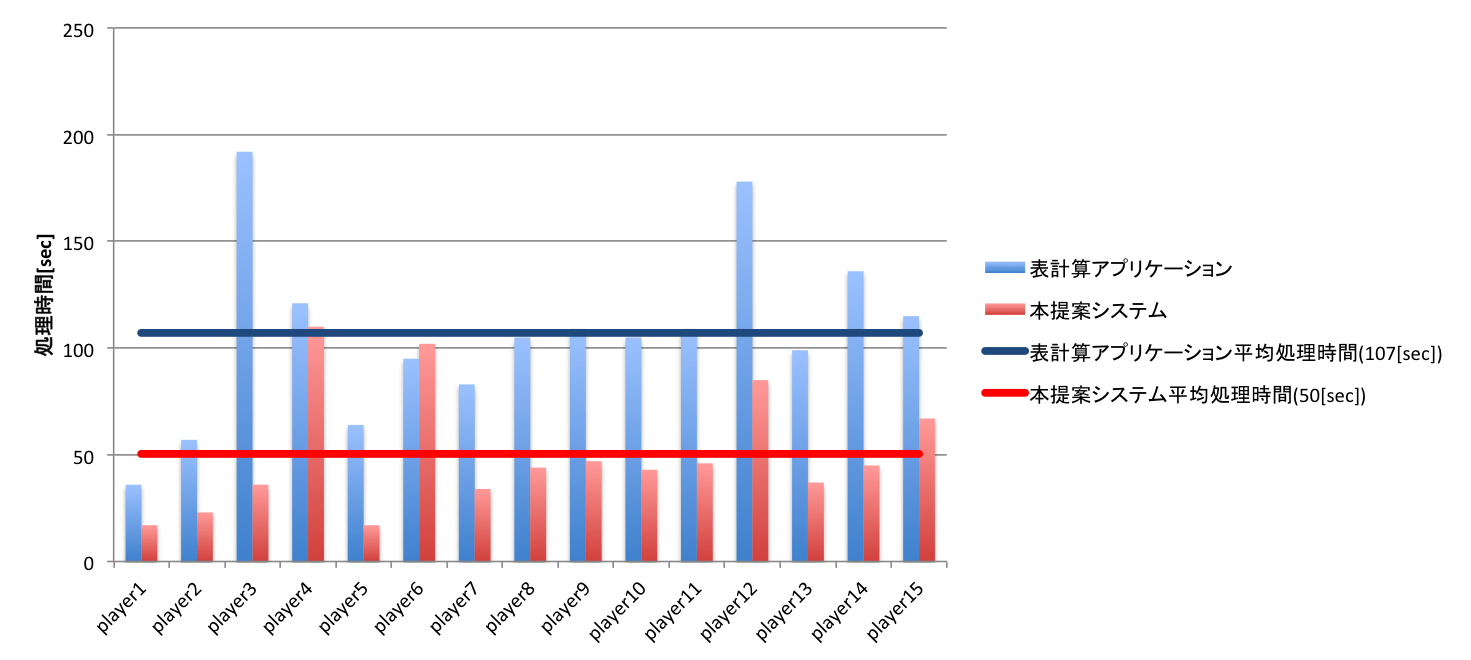
\includegraphics[width=\linewidth]{result03.eps}
				\end{center}
				\caption{本提案システムと、表計算アプリケーションの操作時間}
		  		\label{fig:result03}
			\end{figure}
			\begin{figure}
				\begin{center}
					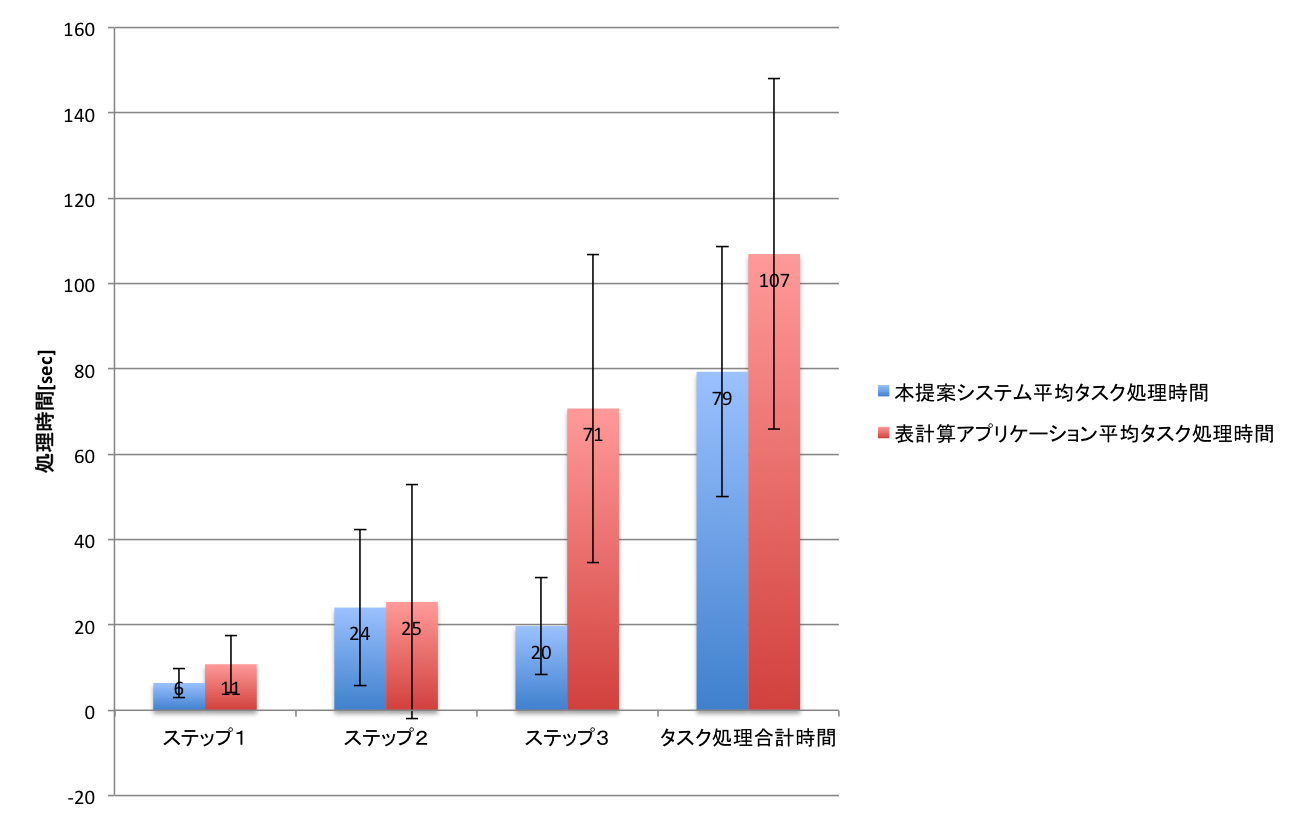
\includegraphics[width=\linewidth]{result04.eps}
				\end{center}
				\caption{本提案システムと、表計算アプリケーションのそれぞれのステップごとの平均処理時間}
		  		\label{fig:result04}
			\end{figure}
			\begin{figure}
				\begin{center}
					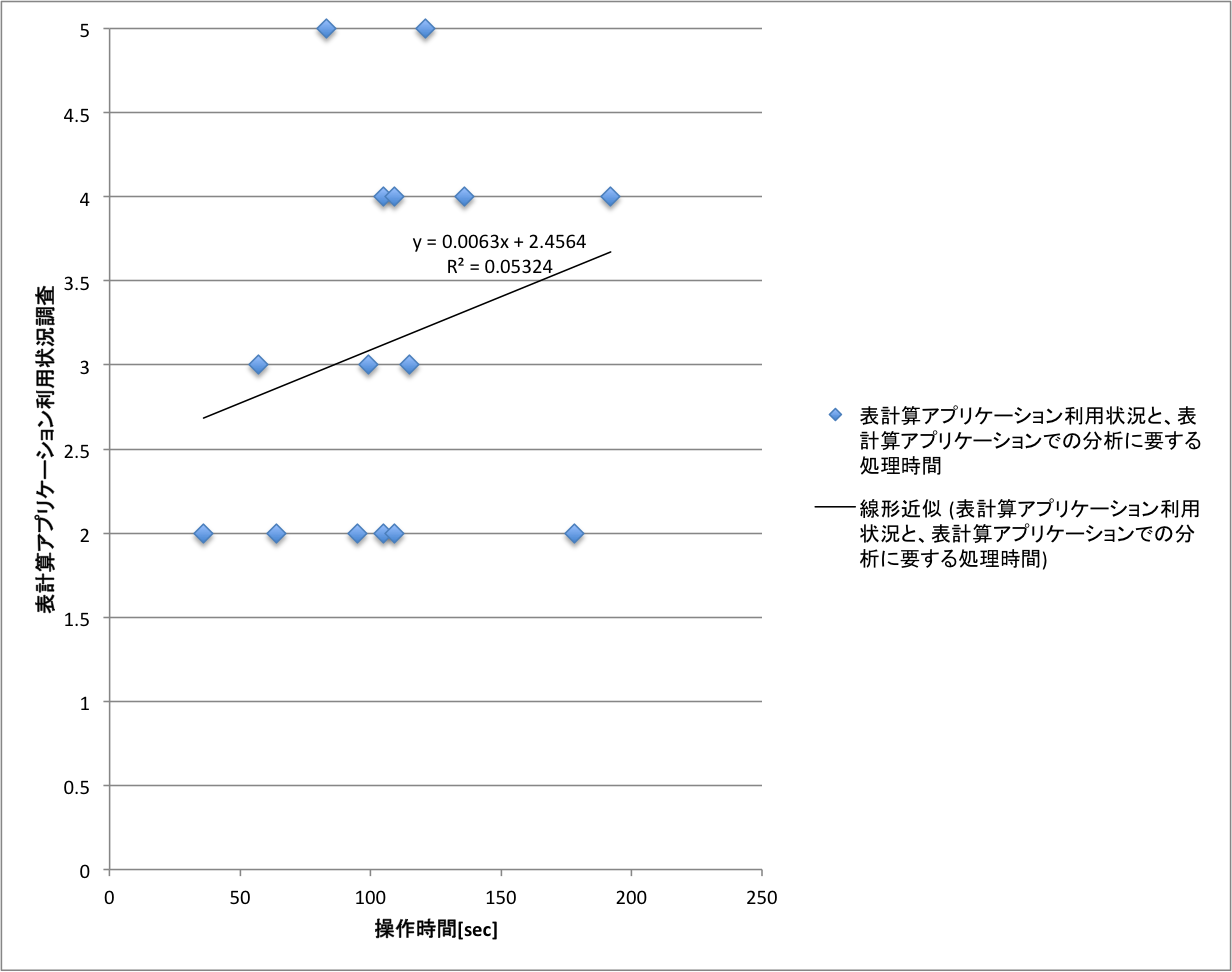
\includegraphics[width=\linewidth]{result05.eps}
				\end{center}
				\caption{表計算アプリケーションでの操作時間と被験者の表計算アプリケーションへの慣れの関係性について}
		  		\label{fig:result05}
			\end{figure}
		\subsection{評価考察}
			\subsubsection{t検定}
				対応のある片側t検定を用いて本提案システムと、表計算アプリケーションによるタスク1の処理時間の検定を行った。
				結果として、p値は6.0E-5となり、本提案システムの優位性が示された。
				一般にp値が0.05以下であれば有意差があるとされている。
			\subsubsection{各ステップでの処理平均時間について}
				各ステップ標準偏差は全般的に本提案システムの方が、表計算アプリケーションより小さい。
				後述するのアンケート結果より、これまで表計算アプリケーションでの分析の利用頻度に差が見られた。表計算アプリケーションでの分析分析していなかった人は、表計算アプリケーションでの処理に時間がかかっているのではないかとも思われたが、図に示すように相関関係は薄く、R\^2=0.054であった。
				表計算アプリケーションでは操作に迷いやすい、もしくは情報探索能力が低いと言える。
				従って、本提案システムは表計算アプリケーションに比べ、だれでも短いタスク処理が可能であると推測される。
	\section{実験3}
		\subsection{実験方法}
			選手が望む利用用途に即した情報探索が可能なシステムになっているか、アンケート調査によって評価した。
			アンケート結果から、t検定を用いて本提案システムと同部で用いられている表計算アプリケーションとの比較をし、有意差があるか調べ、本提案システムの優位性を検証した。
			\\評価実験1,2の後に、アンケート記入を行ってもらった。
			アンケート項目は表に示す。
		\subsection{評価結果}
		アンケート結果を図~\ref{fig:result06}\ref{fig:result07}\ref{fig:result08}に示す。
			\begin{figure}
				\begin{center}
					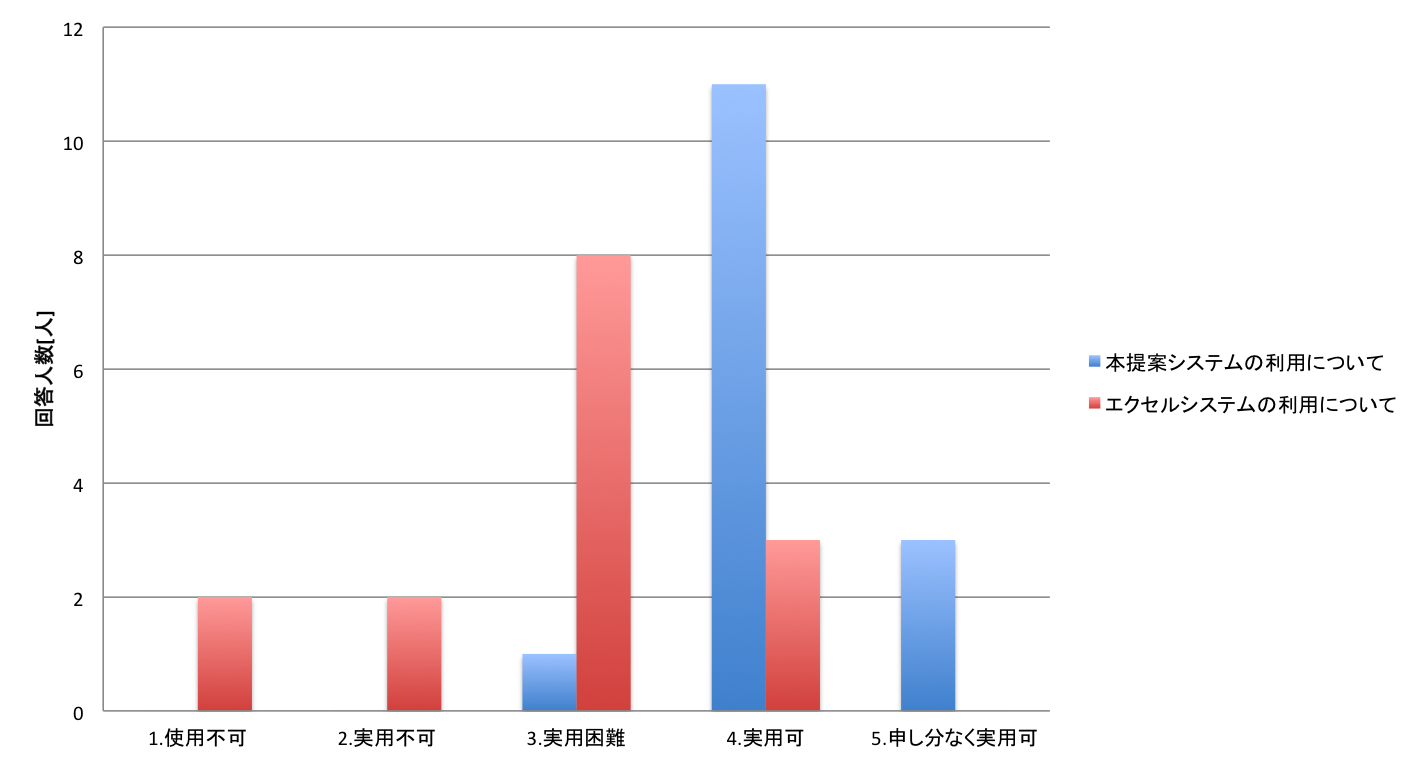
\includegraphics[width=\linewidth]{result06.eps}
				\end{center}
				\caption{実用性について}
		  		\label{fig:result06}
			\end{figure}
			\begin{figure}
				\begin{center}
					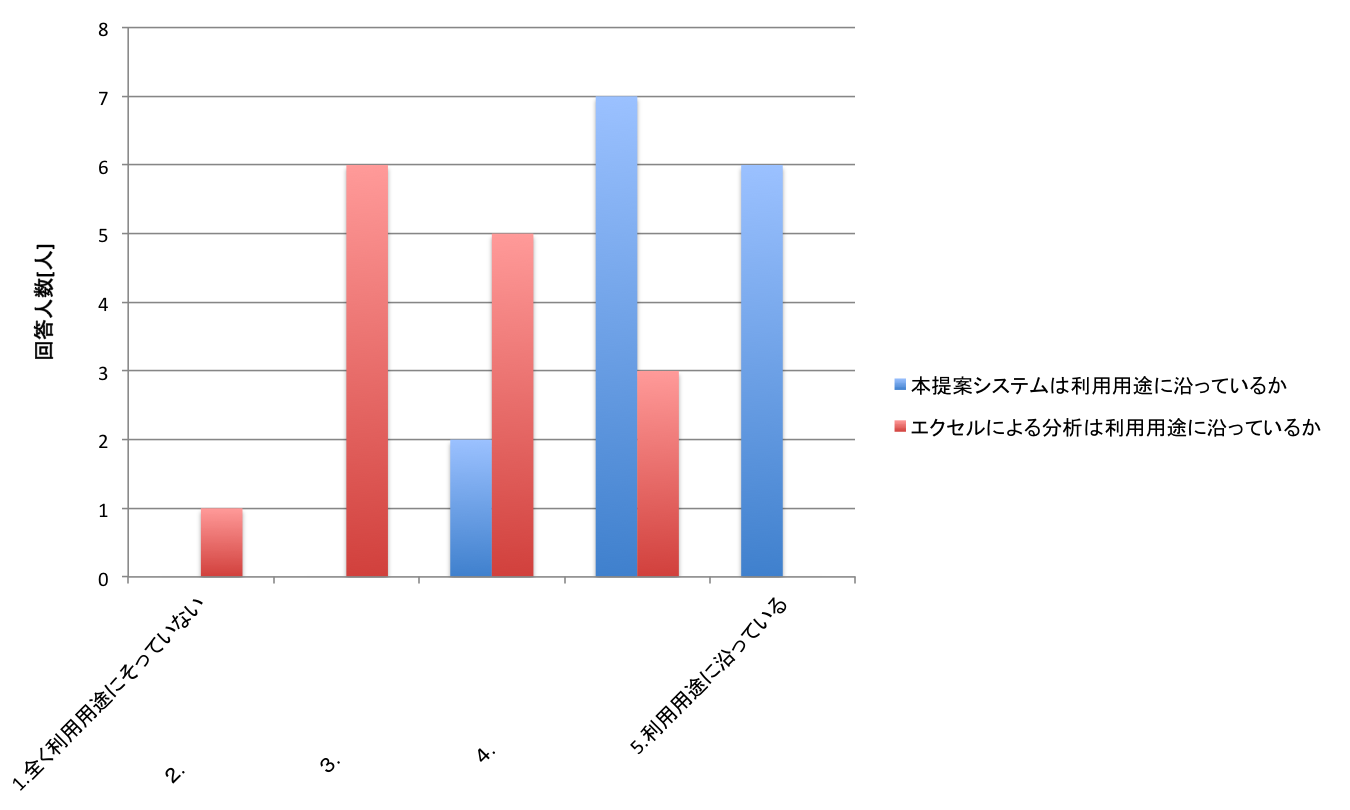
\includegraphics[width=\linewidth]{result07.eps}
				\end{center}
				\caption{利用用途について}
		  		\label{fig:result07}
			\end{figure}
			\begin{figure}
				\begin{center}
					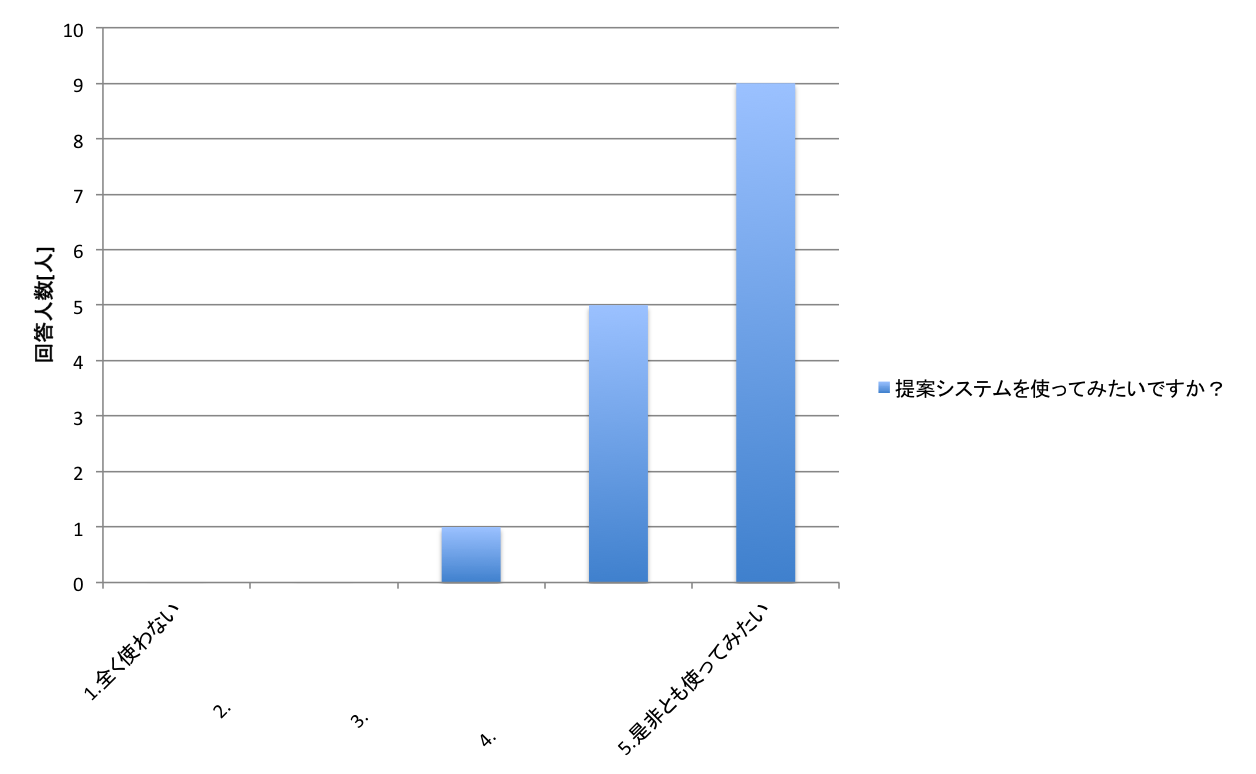
\includegraphics[width=\linewidth]{result08.eps}
				\end{center}
				\caption{提案システムについて}
		  		\label{fig:result08}
			\end{figure}
		\subsection{評価考察}
			アンケートの考察を行う。
			アンケート結果から、対応のある片側t検定を用いて本提案システムと同部で用いられている表計算アプリケーションとの比較を行う。
			本アンケートでは、本提案システムと表計算アプリケーションを用いた分析の利用について利用用途に沿っているか5段階評価を行ったわけだが、この結果を分析するにあたり、対応のある片側t検定を行った。
			結果として、p値1.5E\-6はであった。つまり、表計算アプリケーションによる分析に比べ、本提案システムは利用用途に沿ったシステムであることがわかった。
			同様に実用可能かのアンケートを行ったが、同じくp値は9.4E-6であり、表計算アプリケーションに比べ、実用可能なシステムであることがわかった。

\chapter{結論}


%======================================================================
%		謝辞
%======================================================================
\begin{acknowledgements}
	本研究を進めるにあたり、有益な御指導、御助言を頂きました京都大学高等教育院の小山田耕二教授、坂本尚久特定助教、学際融合教育研究推進センター政策のための科学ユニットの久木元伸如特定講師に深く感謝致します。
	本研究を進めるにあたり、プログラミング技術を始め、様々な御助言を頂きました京都大学工学研究科博士後期課程2年生の尾上洋介氏に深く感謝致します。
	本研究を進めるにあたり、アンケート調査や、システム評価実験に協力して下さった京都大学男子ラクロス部の皆様にはご協力を賜りました。ここに深く御礼申し上げます。
	最後に、家族をはじめとする私の学生生活を支えてくださったすべての皆様へ心から感謝の意を表します。
\end{acknowledgements}



%======================================================================
%		参考文献
%======================================================================
\bibliographystyle{kueethesis}
\bibliography{sample}



%======================================================================
%		付録
%======================================================================
\appendix

%fig



\end{document}
% Local Variables:
% fill-column: 70
% End:
